\section{PWM}

%----------------------------------------------------------------------------------------
%	PWM SUBSECTION
%----------------------------------------------------------------------------------------

\subsection{Definition}
Pulse width modulation (PWM) is a fancy term for describing a type of digital signal. Pulse width modulation is used in a variety of applications including sophisticated control circuitry. A common way we use them here at SparkFun is to control dimming of RGB LEDs or to control the direction of a servo motor. We can accomplish a range of results in both applications because pulse width modulation allows us to vary how much time the signal is high in an analog fashion. While the signal can only be high (usually 5V) or low (ground) at any time, we can change the proportion of time the signal is high compared to when it is low over a consistent time interval.

%----------------------------------------------------------------------------------------
%	DEFINITION SUBSECTION
%----------------------------------------------------------------------------------------
\newpage
\subsection{Duty Cycle}
When the signal is high, we call this “on time”. To describe the amount of “on time” , we use the concept of duty cycle. Duty cycle is measured in percentage. The percentage duty cycle specifically describes the percentage of time a digital signal is on over an interval or period of time. This period is the inverse of the frequency of the waveform.
If a digital signal spends half of the time on and the other half off, we would say the digital signal has a duty cycle of 50\% and resembles an ideal square wave. If the percentage is higher than 50\%, the digital signal spends more time in the high state than the low state and vice-versa if the duty cycle is less than 50\%. Here is a graph that illustrates these three scenarios \\

\centerline{
	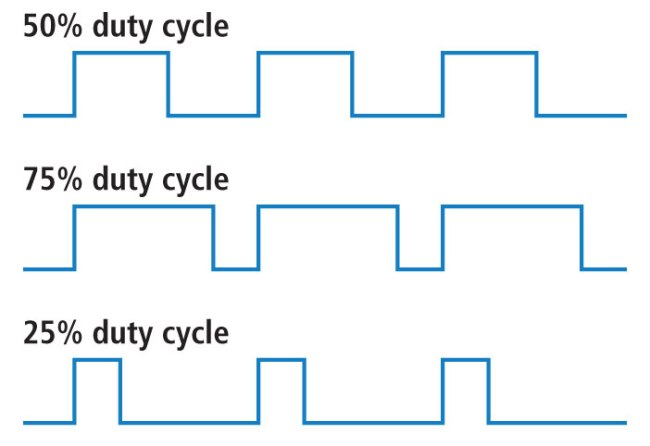
\includegraphics[width=1.0\textwidth]{overview/images/duty.jpg}
}

